\documentclass[a4paper]{article}
\usepackage[pdftex]{graphicx}
\usepackage[utf8]{inputenc}
\usepackage{enumerate}
\usepackage{siunitx}
\sisetup{locale=DE} 
\usepackage{icomma}
\usepackage{amssymb}
\usepackage{tikz}
\usepackage{href-ul}
\hypersetup{
	colorlinks=true,
	linkcolor=blue,
	urlcolor=blue}
\usepackage{geometry}
\geometry{a4paper, top=15mm, left=15mm, right=15mm, bottom=15mm,
	headsep=10mm, footskip=12mm}

\begin{document}
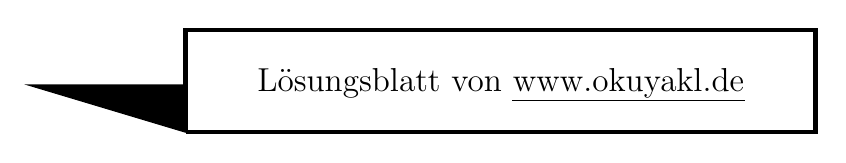
\begin{tikzpicture}(10,3)
	\draw[ultra thick](2,0) --(10,0) -- (10,1.3) --(2,1.3) -- (2,0);
	\draw[fill=black](2,0)-- (0,.6) -- (2,.6) -- (2,0);
	\node at (6,.6) {\large Lösungsblatt von \href{https://www.okuyakl.de}{www.okuyakl.de}};
\end{tikzpicture}
\vspace{0.5 cm}

\noindent{\bf Aufgabe 1.}\\
\begin{minipage}{0.7\textwidth}
	Das Dreieck, dass durch die Vektoren der Gewichtskraft $F_G$ und der Hangabtriebskraft $F_H$ aufgespannt ist, ist ähnlich zu dem Dreieck der Rampe mit der Länge $l$ und der Höhe $h$. Dies bedeutet für das Verhältnis der Beträge der Kräfte gilt:
	$${F_H \over F_G}={h \over l}$$
	Die Hangabtriebskraft ist die Gegenkraft der Zugkraft $F_Z$ und wir können sie mit ihr gleichsetzen. Damit folgt:
	$$F_Z = F_H = {h \over l}\cdot F_G = {\SI{1,2}{\meter} \over \SI{3,0}{\meter}}\cdot \SI{600}{\newton} =\SI{240}{\newton}$$
\end{minipage}
\begin{minipage}{0.3\textwidth}
	\includegraphics[width=6 cm]{fass122}
\end{minipage}

\noindent
\fbox{
\begin{minipage}{0.4\textwidth}
	\noindent{\bf Aufgabe 2. a)}
	Die Steigung ist 10 \% , also überwindet der LKW einen Höhenunterschied von
	$$h= \SI{20000}{\meter} \cdot 0,1 = \SI{2000}{\meter}$$ 
	
	\noindent{\bf Aufgabe 2. b)}
	Weil der Neigungswinkel klein ist, kann näherungsweise die Zugkraft $F_Z$ aus der Gewichtskraft und der Neigung berechnet werden:
	$${F_Z \over F_G}=0,1 \quad \Rightarrow \quad F_Z = m \cdot g \cdot 0,1$$
	$$F_Z= \SI{27,5}{\kilo\newton}$$ 

\end{minipage}}
\hfill
\fbox{
\begin{minipage}{0.5\textwidth}
\noindent{\bf Aufgabe 3}\\
	\setlength{\unitlength}{1 cm}
	\begin{picture}(7,10)
	\put(0,9){\circle*{0.2}}
	\put(0,6){\circle*{0.2}}
	\put(4,6){\circle*{0.2}}
	\put(0,6){\line(1,0){4}}
	\put(0,9){\line(4,-3){4}}
	\put(2,6){\vector(0,-1){5.2}}
	\put(4,6){\vector(0,-1){2.6}}
	\put(4,6){\vector(4,-3){3,47}}
	\put(4,3.4){\line(1,0){3.47}}
	\put(2.1,4.2){$\vec{F_G}$}
	\put(6,5){$\vec{F_S}$}
	\put(0,9.2){A}
	\put(0,6.2){C}
	\put(4,6.2){B}
	\end{picture}\\
	Wir lesen ab: $F_S=\SI{43}{\newton}$
\end{minipage}
}


\noindent {\bf Aufgabe 4. a)}\\
Diese Aufgabe ist zeichnerisch zu lösen, ohne Trigonometrie.
Im Kräfteplan hier wird Viola als Massepunkt dargestellt. Ihre Gewichtskraft beträgt $F=\SI{9,81}{\meter\over \second^2}\cdot \SI{51}{\kilogram}  = \SI{500}{\newton} $. $\SI{1}{\centi\meter}$ entspricht $\SI{10}{\newton}$.\\

\begin{minipage}{0.5\textwidth}
\setlength{\unitlength}{1 cm}
\begin{picture}(7,7)
\put(4,5.5){\circle*{0.2}}
\put(4,5.5){\vector(0,-1){5}}
\put(4,5.5){\vector(-4,-3){2.4}}
\put(4,5.5){\vector(3,-4){2.4}}
\put(0.5,2.5){\line(1,0){6}}
\put(0.5,2.5){\line(4,3){6}}
\put(6.5,2.5){\line(0,1){4.5}}
\put(4,0.5){\line(4,3){2.4}}
\put(4,0.5){\line(-3,4){2.4}}
\put(4.2,3){$\vec{F_G}$}
\put(2.5,5){$\vec{F_H}$}
\put(5,4.2){$\vec{F_N}$}
\end{picture}
\end{minipage}
\begin{minipage}{0.5\textwidth}
\noindent {\bf Aufgabe 4. b)}\\
Aus dem Kräfteplan lesen wir die Hangabtriebskraft $\vec{F_H}$ ab: 

$$\vec{F_H}=\SI{300}{\newton} $$
$$ a = {F_H \over m} = { \SI{300}{\newton} \over \SI{51}{\kilogram} }= \SI{5,9}{\meter\over {\second^2}}$$

\noindent {\bf Aufgabe 4. c)}\\
Die Reibungskraft berechnet sich aus der Reibungszahl $\mu$ und der Normalkraft $\vec{F_N}$.
$$ \vec{F_R}= \mu \cdot \vec{F_N}$$

\noindent Für die resultierende Beschleunigung gilt: 
$$ a_R = \frac{F_H - F_R}{m}= {\SI{300}{\newton} - 0,15 \cdot \SI{400}{\newton} \over \SI{51}{\kilogram} } = \SI{4,7}{\meter\over {\second^2}}$$ 
\end{minipage}

\begin{center}
	\includegraphics[width=7 cm]{../../viecher/endcomic.pdf}
	
	Hier geht es zurück zum \href{https://www.okuyakl.de/phys/p9kraL404/aa404.pdf}{Aufgabenblatt}
\end{center}


\end{document}

